\documentclass[a4paper]{article}

%% Language and font encodings
\usepackage[english]{babel}
\usepackage[utf8x]{inputenc}
\usepackage[T1]{fontenc}

%% Sets page size and margins
\usepackage[a4paper,top=3cm,bottom=2cm,left=3cm,right=3cm,marginparwidth=1.75cm]{geometry}

%% Useful packages
\usepackage{amsmath}
\usepackage{graphicx}
\usepackage[colorinlistoftodos]{todonotes}
\usepackage[colorlinks=true, allcolors=blue]{hyperref}
\usepackage{prooftree,amsmath,amssymb,xcolor,wasysym,xspace,url}
\usepackage{mathptmx}
\usepackage{stmaryrd}
\usepackage{tikz}

\newif\ifhasadjustbox
\IfFileExists{adjustbox.sty}{%
  \usepackage{adjustbox}
  \hasadjustboxtrue
}{%
  \hasadjustboxfalse
}%

\newif\ifhasadjustbox
\IfFileExists{adjustbox.sty}{%
  \usepackage{adjustbox}
  \hasadjustboxtrue
}{%
  \hasadjustboxfalse
}


%\newcommand{\labelx}[1]{\label{#1}($#1$)}
\newcommand{\labelx}[1]{\label{#1}}
\newcommand{\ruler}[1]{\hbox{[#1]}}
\newcommand{\rulename}[1]{[\textsc{\small #1}]}
\newcommand{\xlbranch}[3]{\ensuremath{#1 {\&} ({#2}, {#3})}}
\newcommand{\xlsel}[3]{\xlselp{#1}{#2}{#3}.}
\newcommand{\xlselp}[3]{\ensuremath{#1 {\oplus} \anglep{#2}{#3}}}
%SINTASSI
\newcommand{\upd}{\mathit{update}}
\newcommand{\pn}{\p}
\newcommand{\rtsyntax}[1]{%
        \adjustbox{bgcolor=lightgray,bgcolor=lightgray}{\strut\ensuremath{\,#1\,}}%
}
%\newcommand{\rtsyntax}[1]{\colorbox{lightgray}{\ensuremath{#1}}}
\newcommand{\ptilde}[1]{{\ensuremath{#1}}}
%\newcommand{\kf}[1]{\textsf{\upshape\small #1}\xspace}
\newcommand{\kf}[1]{\textup{\textsf{#1}}\xspace}
\newcommand{\constf}[1]{\textup{\textsf{#1}}}
\newcommand{\srsimple}[3]{\ensuremath{\bar{#1}[#2](#3)}}
\newcommand{\sr}[4]{\ensuremath{\srsimple{#1}{#2}{#3}.#4}}
\newcommand{\uu}{\ensuremath{u}}
\newcommand{\Ia}{\ensuremath{a}}
\newcommand{\Ic}{\ensuremath{c}}
\newcommand{\Ias}{\ensuremath{\alpha}}
\newcommand{\Ib}{\ensuremath{b}}
\newcommand{\y}{\ensuremath{y}}
\newcommand{\PP}{\ensuremath{P}}
\newcommand{\Q}{\ensuremath{Q}}
\newcommand{\R}{\ensuremath{R}}
\newcommand{\DD}{\ensuremath{D}}
\newcommand{\sasimple}[3]{\ensuremath{#1[#2](#3)}}
\newcommand{\sa}[4]{\ensuremath{\sasimple{#1}{#2}{#3}.#4}}
\newcommand{\pp}{\ensuremath{\at{\p}}}
\newcommand{\si}[2]{\ensuremath{#1[#2]}}
\newcommand{\sI}[1]{\ensuremath{\s_{#1}}}
%\newcommand{\sI}[1]{\ensuremath{\s^#1}}   vecchia versione
\newcommand{\sii}{\si{\s}{\p}}
\newcommand{\sij}{\si{\s}{\p_j}}
\newcommand{\siq}{\si{\s}{\q}}
\newcommand{\siip}{\si{\s'}{\p'}}
\newcommand{\sipp}{\si{\s'}{\p}}
\newcommand{\cc}{\ensuremath{c}}
\newcommand{\pset}{\ensuremath{\Pi}}
\newcommand{\inpset}[2][\Pi]{\ensuremath{\p_#2 \in #1}}
\newcommand{\kinpset}{\inpset{k}}
%\newcommand{\pset}{\ensuremath{\set{\participant{\p}_k}_{k\in K}}}
\newcommand{\out}[4]{\ensuremath{#1!\langle #2,#3\rangle.#4}}   %--M
%\newcommand{\out}[4]{\ensuremath{#1!\langle \set{#3_k}_{k\in K},#2\rangle;#4}}
%\newcommand{\outp}[3]{\ensuremath{#1!\langle \pset,#2\rangle}}  ---M
\newcommand{\outp}[3]{\ensuremath{#1!\langle \p,#2\rangle}}    %--M
\newcommand{\outs}[4]{\ensuremath{#1!\langle #3,#2\rangle.#4}}
\newcommand{\e}{\ensuremath{e}}
\newcommand{\inp}[4]{\ensuremath{#1?( #3,#2).#4}}
\newcommand{\inpp}[3]{\ensuremath{#1?( #3,#2)}}
\newcommand{\inps}[4]{\ensuremath{#1?( #3,#2).#4}}
\newcommand{\x}{\ensuremath{x}}
\newcommand{\participant}[1]{\ensuremath{\mathtt{#1}}}
\newcommand{\q}{\ensuremath{\participant{q}}}
\newcommand{\p}{\ensuremath{\participant{p}}}
\newcommand{\sd}[4]{\ensuremath{#1!\langle\! \langle#3,#2\rangle \!\rangle.#4}}
\newcommand{\sdsp}[3]{\ensuremath{#1!\langle\! \langle#3,#2\rangle \!\rangle}}
\newcommand{\sdt}[4]{\ensuremath{#1^\top!\langle\! \langle#3,#2\rangle \!\rangle.#4}}
\newcommand{\sdp}[3]{\ensuremath{#1!\langle\! \langle#3,#2\rangle \!\rangle}}
\newcommand{\rdp}[3]{\ensuremath{#1?(\!(#3,#2)\!)}}
%\newcommand{\sdp}[4]{\ensuremath{#1!^{\lev'}\langle\! \langle#3,#2\rangle \!\rangle.#4}}
\newcommand{\rd}[4]{\ensuremath{#1?(\!(#3,#2)\!).#4}}
\newcommand{\rdt}[4]{\ensuremath{#1^\top?(\!(#3,#2)\!).#4}}
\newcommand{\z}{\ensuremath{z}}
\newcommand{\pc}{\Par}
\newcommand{\s}{\ensuremath{s}}
\newcommand{\X}{\ensuremath{X}}
\newcommand{\defX}{\ensuremath{\kf{def} \ \Ddef\ \kf{in}\ }}
\newcommand{\Xsignature}{\ensuremath{\X(\x, \y)}}
\newcommand{\Xsignaturep}{\ensuremath{\X(\x, \y')}}
\newcommand{\Ddef}{\ensuremath{\Xsignature=\PP}}
\newcommand{\Ddefp}{\ensuremath{\Xsignature=\PP'}}
\newcommand{\DdefpO}{\ensuremath{\Xsignature=\PP_0}}
\newcommand{\Ddefpp}{\ensuremath{\Xsignature=\R}}
\newcommand{\defIn}[1]{\ensuremath{\kf{def} \ #1 \ \kf{in}\ }}
\newcommand{\defD}{\ensuremath{\kf{def}\ \DD \ \kf{in}\ }}
\newcommand{\DdefD}{\ensuremath{\kf{def}\ \Ddef \ \kf{in}\ }}
\newcommand{\defDp}{\ensuremath{\kf{def}\ \DD' \ \kf{in}\ }}
\newcommand{\proccall}[3]{\ensuremath{#1\langle\ptilde{#2},\ptilde{#3}\rangle}}
\newcommand{\proccallw}[3]{\ensuremath{#1\langle\ptilde{#2},\ptilde{#3}\rangle}}
\newcommand{\proccalldots}[3]{\ensuremath{#1\langle\ptilde{#2},\ptilde{#3}\rangle}}

\newcommand{\indexed}[4]{\ensuremath{\{#1_#3 : #2_#3\}_{#3 \in #4}}}

\newcommand{\values}{\ensuremath{\at{v}}}
\newcommand{\trival}[3]{\ensuremath{(#3,#2, #1)}}
\newcommand{\labval}[2]{\ensuremath{(#1, #2)}}
\newcommand{\anglep}[2]{\ensuremath{\langle #1, #2\rangle}}
\newcommand{\valheap}[3]{\ensuremath{( #3,#2,#1 )}}    %--M
\newcommand{\valheaps}[3]{\ensuremath{( #3,#2,#1 )}}
\newcommand{\valheapj}[2]{\ensuremath{( #2,\{j\},#1 )}}
%\newcommand{\valheapp}[2]{\ensuremath{( #2,\{\p\},#1 )}}
\newcommand{\valheapp}[2]{\ensuremath{( #2,\p,#1 )}}
\newcommand{\valheapLess}[3]{\ensuremath{( #3,\pset\setminus \p,#1 )}}
\newcommand{\delheap}[3]{\ensuremath{(#3,{#2},#1 )}}
\newcommand{\labheap}[3]{\ensuremath{( #3,#2,#1 )}}    %--M
\newcommand{\labheaps}[3]{\ensuremath{( #3,#2,#1 )}}
\newcommand{\labheapj}[2]{\ensuremath{( #2,\{j\},#1 )}}
%\newcommand{\labheapp}[2]{\ensuremath{( #2,\{\p\},#1 )}}
\newcommand{\labheapp}[2]{\ensuremath{( #2,\p,#1 )}}
\newcommand{\lsel}[4]{\ensuremath{#1 \oplus \anglep{#2}{#3}.#4}}   %--M
\newcommand{\sel}[4]{\ensuremath{#1 \oplus \anglep{#3}{#2}.#4}}
\newcommand{\lbranch}[2]{\ensuremath{#1 \&
({#2},\indexed{l}{\PP}{i}{I})}}
\newcommand{\lbranchR}[2]{\ensuremath{#1 \&
({#2},\indexed{l}{\R}{i}{I})}}
\newcommand{\lbranchi}[2]{\ensuremath{#1 \&
({#2},\indexed{l}{\PP}{i}{I})}}

%\newcommand{\ifthenelse}[3]{\ensuremath{\kf{if}\ #1\ \kf{then}\ #2\ \kf{else}\ #3}}
\newcommand{\inact}{\ensuremath{\mathbf{0}}}
\newcommand{\nuc}[2]{\ensuremath{(\nu #1)#2}}
\newcommand{\AND}[2]{\ensuremath{#1\ \kf{and}\ #2}}
\newcommand{\NOT}[1]{\ensuremath{\kf{not}\ #1}}
\newcommand{\true}{\kf{true}}
\newcommand{\false}{\kf{false}}
\newcommand{\h}{\ensuremath{h}}
\newcommand{\mg}{\ensuremath{m}}
\newcommand{\va}{\ensuremath{v}}
\newcommand{\at}[1]{\ensuremath{\ptilde{#1}}}
\newcommand{\atw}[1]{\ensuremath{\ptilde{#1}}}
\newcommand{\Co}[1]{\ensuremath{C[#1]}}
\newcommand{\Par}{\ensuremath{\ |\ }}
\newcommand{\cas}{\ensuremath{r}}
\newcommand{\eq}{\ensuremath{\diameter}}

%SEMANTICA
\newcommand{\redsym}{\ensuremath{\longrightarrow}}
\newcommand{\red}[2]{\ensuremath{#1\redsym#2}}
\newcommand{\redM}[2]{\ensuremath{#1\redsym^*#2}}
\newcommand{\redN}[2]{\ensuremath{#1\redsym^n#2}}
\newcommand{\redK}[2]{\ensuremath{#1\redsym^k#2}}
\newcommand{\redP}[2]{\ensuremath{#1\redsym^+#2}}
\newcommand{\set}[1]{\ensuremath{\{#1\}}}
\newcommand{\mset}[1]{\ensuremath{\{\!\!\{#1\}\!\!\}}}
\newcommand{\sub}[2]{\ensuremath{\{#1/#2\}}}
\newcommand{\ssub}[2]{\ensuremath{\{#1/#2\}}}
\newcommand{\subO}[2]{\ensuremath{\set{\!\{#1/#2\}\!}}}

\newcommand{\sep}{\ensuremath{~\mathbf{|\!\!|}~ }}

\newcommand{\Implies}{\ensuremath{\quad \Rightarrow \quad }}

\newcommand{\mqueue}[2]{\ensuremath{#1 : #2}}
\newcommand{\emptyqueue}[1]{\mqueue{\s}{\emptyset}}
\newcommand{\queue}{\ensuremath{\h}}
\newcommand{\stdqueue}{\mqueue{\s}{\queue}}
\newcommand{\qcomp}[2]{\ensuremath{#1 \cdot #2}}
\newcommand{\qtail}[1]{\ensuremath{\qcomp{\queue}{#1}}}
\newcommand{\qhead}[1]{\ensuremath{\qcomp{#1}{\queue}}}
\newcommand{\qm}[1]{\ensuremath{\qcomp{\queue_1}{\qcomp{#1}{\queue_2}}}}

\newcommand{\qappend}[1]{\mqueue{\s}{\qtail{#1}}}
\newcommand{\qpop}[1]{\mqueue{\s}{\qhead{#1}}}

\newcommand{\subst}[2]{\ensuremath{\{#1 / #2\}}}
\newcommand{\remove}[2]{\ensuremath{#1 \backslash \{#2\}}}

\newcommand{\freen}[1]{\ensuremath{\text{fn}(#1)}}
\newcommand{\dpv}[1]{\ensuremath{\text{dpv}(#1)}}
\newcommand{\fpv}[1]{\ensuremath{\text{fpv}(#1)}}
\newcommand{\rrule}[1]{[\text{#1}]}

%TIPI
\newcommand{\G}{\ensuremath{G}}
\newcommand{\Gv}[4]{\ensuremath{#1\to #2:\langle#3\rangle.#4}}  %--M
\newcommand{\Gvr}[4]{\ensuremath{#1\to#2:\langle#3\rangle.#4}}
\newcommand{\U}{\ensuremath{U}}
\newcommand{\sid}[1]{\ensuremath{\textup{mp}(#1)}}
\newcommand{\pro}[2]{\ensuremath{#1\upharpoonright#2}}
\newcommand{\Ga}{\ensuremath{\Gamma}}
\newcommand{\D}{\ensuremath{\Delta}}
\newcommand{\Dp}{\ensuremath{\D'}}
\newcommand{\T}{\ensuremath{T}}
\newcommand{\TQ}{\ensuremath{{M}}}     % {\ensuremath{{\tt{T}}}}
\newcommand{\TG}{\ensuremath{{\tau}}}   %{\ensuremath{{\mathsf{T}}}}
\newcommand{\TGP}{\ensuremath{{\mathfrak{T}}}}
\newcommand{\Tp}{\ensuremath{T'}}
\newcommand{\ST}{\ensuremath{S}}
\newcommand{\TT}{\atw{\T}}
\newcommand{\SST}{\atw{S}}
\newcommand{\UT}{\ensuremath{U}}
\newcommand{\oT}[2]{\ensuremath{{!}\langle #2,#1\rangle}}
%\newcommand{\sTm}{\ensuremath{\not\;!}}
\newcommand{\sTm}{\ensuremath{!}}
\newcommand{\oTm}[2]{\ensuremath{\;\sTm\langle #2,#1\rangle}}
\newcommand{\iT}[2]{\ensuremath{?( #2,#1 )}}
\newcommand{\iTs}[2]{\ensuremath{\&( #2,#1 )}}
\newcommand{\oTG}[2]{\ensuremath{\;\natural\langle #2,#1\rangle}}
\newcommand{\oTGp}[2]{\ensuremath{\;\natural'\langle #2,#1\rangle}}
%\newcommand{\an}[1]{\ensuremath{\langle #1\rangle}}
\newcommand{\an}[1]{\ensuremath{ #1}}
\newcommand{\de}[3]{\ensuremath{#1\vdash#2:#3}}
\newcommand{\der}[3]{\ensuremath{#1\vdash#2\triangleright#3}}
\newcommand{\derl}[3]{\ensuremath{#1\vdash^\leq#2\triangleright#3}}
\newcommand{\dom}[1]{\ensuremath{dom( #1)}}
\newcommand{\range}[1]{\ensuremath{range( #1)}}
\newcommand{\ty}{\textbf{t}}
\newcommand{\End}{\kf{end}}
\newcommand{\Bool}{\kf{bool}}
\newcommand{\Nat}{\kf{nat}}
%\newcommand{\setk}[1]{\ensuremath{\set{#1_k}_{k\in K}}}

\newcommand{\SelType}[2]{\ensuremath{\oplus(#1,#2)}}

\newcommand{\seltype}{\ensuremath{\oplus \langle \p,\{l_i:\T_i\}_{i\in
I} \rangle }}   %--M
\newcommand{\seltypeP}[1]{\ensuremath{\oplus \langle #1,\{l_i:\T_i\}_{i\in
I} \rangle }}   %--M
\newcommand{\seltypeCl}{\ensuremath{\oplus \langle \pset,\{l_i:\cloT_i\}_{i\in
I} \rangle }}
\newcommand{\seltypeph}{\ensuremath{\oplus \langle \pset,\{l_i:\hat\T_i\}_{i\in
I} \rangle }}
\newcommand{\seltypeC}{\ensuremath{\oplus \langle \pset,\{l:\calT,l_i:\T_i\}_{i\in
I} \rangle }}
\newcommand{\seltypeG}{\ensuremath{\oplus(\p,\{l_i:\pro{\G_i}\q\}_{i\in I})}}
\newcommand{\seltypeT}{\ensuremath{\oplus\{l_i:\pro{\T_i}\q\}_{i\in I}}}
\newcommand{\seltypeTprf}{\ensuremath{\oplus\{l_i:\TGP_i\}_{i\in I}}}
\newcommand{\seltypeTp}{\ensuremath{\oplus\{l_i:\T_i\}_{i\in I}}}
\newcommand{\seltypeq}{\ensuremath{\oplus\langle\pset,l\rangle;\T}}
\newcommand{\seltypeqg}{\ensuremath{\oplus\langle\pset,l\rangle;\TG}}
\newcommand{\seltypeqj}{\ensuremath{\oplus\langle\{j\},l\rangle;\T}}
\newcommand{\seltypeqq}{\ensuremath{\oplus\langle\q,l\rangle;\T}}
\newcommand{\seltypeqqG}{\ensuremath{\oplus\langle\q,l\rangle;\TG}}
\newcommand{\seltypep}{\ensuremath{\oplus(\pset,l);\T'}}
\newcommand{\seltypezp}{\ensuremath{\oplus(\pset,l:\T_0;\T')}}
\newcommand{\seltypez}{\ensuremath{\oplus(\pset,l:\T_0)}}
\newcommand{\seltypei}{\ensuremath{\oplus\langle\pset,l_i\rangle;\T_i}}
\newcommand{\seltypej}{\ensuremath{\oplus(\p,l_j);\T_j}}    %--M
\newcommand{\seltypesi}{\ensuremath{\oplus(\p,l_{i})}}    %--M
\newcommand{\seltypesip}{\ensuremath{\oplus(\pset,l_{i'})}}
\newcommand{\seltypesipz}{\ensuremath{\oplus(\pset,l_{i_0})}}
\newcommand{\seltypesipzs}{\ensuremath{\oplus(\set\p,l_{i_0})}}
\newcommand{\seltypesipzsj}{\ensuremath{\oplus\langle\p,l_j\rangle}}
\newcommand{\seltypesipjz}{\ensuremath{\oplus(\pset\setminus \p,l_{i_0})}}
\newcommand{\seltypesipj}{\ensuremath{\oplus(\pset\setminus \p,l_{i'})}}
\newcommand{\seltypes}{\ensuremath{\oplus\langle\p,l\rangle}}  %--M
\newcommand{\seltypesq}{\ensuremath{\oplus\langle\q,l\rangle}}  %--M
\newcommand{\seltypesj}{\ensuremath{\oplus\langle\pset,l_j\rangle}}
\newcommand{\seltypesem}{\ensuremath{\oplus(\emptyset,l)}}
\newcommand{\seltypesemZ}{\ensuremath{\oplus(\emptyset,Z)}}
\newcommand{\branchtype}{\ensuremath{\&(\p,\{l_i:\T_i\}_{i\in I})}}
\newcommand{\branchtypeCl}{\ensuremath{\&(\p,\{l_i:\cloT_i\}_{i\in I})}}
\newcommand{\branchtypeqq}{\ensuremath{\&(\p,\{l_i:\T^{(\q)}_i\}_{i\in I})}}
\newcommand{\branchtypeqqh}{\ensuremath{\&(\p,\{l_i:\hat\T^{(\q)}_i\}_{i\in I})}}
\newcommand{\branchtypeC}{\ensuremath{\&(\p,\{l:\calT,l_i:\T_i\}_{i\in I})}}
\newcommand{\branchtypeq}{\ensuremath{\&(\q,\{l_i:\T_i\}_{i\in I})}}
\newcommand{\branchtypeG}{\ensuremath{\&(\p,\{l_i:\pro{\G_i}\q\}_{i\in I})}}
\newcommand{\branchtypeT}{\ensuremath{\&\{l_i:\pro{\T_i}\q\}_{i\in I}}}
\newcommand{\branchtypeTp}{\ensuremath{\&\{l_i:\T'_i\}_{i\in I}}}
\newcommand{\branchtypeTprf}{\ensuremath{\&\{l_i:\TGP'_i\}_{i\in I}}}
\newcommand{\branchtypes}{\ensuremath{\&\{l_i:\T_i\}_{i\in I}}}
\newcommand{\branchtypepf}{\ensuremath{\&\{l_i:\TGP_i\}_{i\in I}}}
\newcommand{\branchtypesG}{\ensuremath{\&\{l_i:\TG_i\}_{i\in I}}}

\newcommand{\Xtype}{\ensuremath{\X : \SST\;\TT}}
\newcommand{\XtypeP}{\ensuremath{\X : \SST\;\ty}}
\newcommand{\XtypeQ}{\ensuremath{\X : \SST\;\mu\ty.\TT}}

\newcommand{\trule}[1]{\ensuremath{(\text{\sc{#1}})}}
\newcommand{\ins}{\ensuremath{:}}
\newcommand{\equivT}[2]{\ensuremath{#1\approx #2}}
% TIPI CODA
\newcommand{\derqq}[4]{\ensuremath{#1 \vdash_{#2} #3 \triangleright #4}}
\newcommand{\derq}[3]{\ensuremath{#1 \vdash_{\set\s} #2 \triangleright #3}}
\newcommand{\ms}[2]{\ensuremath{{#1}\setminus{#2}}}
\newcommand{\coe}[2]{\ensuremath{\mathsf{co}({#1},{#2})}}
\newcommand{\Ltypes}{\mathcal{L}_{\T}}
\newcommand{\Qtypes}{\mathcal{Q}_{\T}}
\newcommand{\Dcomp}{\ensuremath{\ast}}
\newcommand{\Tcomp}{\ensuremath{;}}
\newcommand{\dual}[2]{\ensuremath{{#1}\bowtie{#2}}}
\newcommand{\dualIO}[2]{\ensuremath{{#1}~\mf{\stackrel{-}{\Bowtie}}~{#2}}}
%INVERSIONE
\newcommand{\ifthen}[2]{If {#1}, then {#2}.}
\newcommand{\cleq}{\ensuremath{\sqsubseteq}}
\newcommand{\sered}[2]{\ensuremath{{#1}~\Rightarrow~{#2}}}
\newcommand{\seredstar}[2]{\ensuremath{{#1}~\Rightarrow^*~{#2}}}
%PROGRESSO

\newcommand{\cu}{\ensuremath{\lambda}}
\newcommand{\cuu}{\ensuremath{\lambda'}}
\newcommand{\B}{\ensuremath{\mathcal{B}}}
\newcommand{\M}{\ensuremath{\mathcal{N}}}
\newcommand{\n}{n}
\newcommand{\Or}{\ensuremath{\mathcal{R}}}
\newcommand{\Se}{\ensuremath{\mathcal{S}}}
\newcommand{\V}{\ensuremath{\mathcal{V}}}
\newcommand{\Th}{\ensuremath{\Theta}}
\newcommand{\semicolumn}{\textup{\texttt{;}}}
\newcommand{\dere}[2]{\ensuremath{\Th\,;\Or;\,\M\,;\,\B\vdash #1\; \blacktriangleright\; #2}}
\newcommand{\dereprime}[1]{\ensuremath{\Th\,\vdash #1\; \blacktriangleright\;
\Or' \,;\,\M'\,;\,\B'}}
\newcommand{\dereb}[3]{\ensuremath{\Th\,\vdash #1 \;\blacktriangleright\; #2 \,;\,\M\,;\,#3}}
\newcommand{\derep}[4]{\ensuremath{#1\,\vdash #2 \;\blacktriangleright\; #3 \,;\;#4\,;\;\B}}
\newcommand{\derepb}[5]{\ensuremath{#1\,\vdash #2 \;\blacktriangleright\; #3 \,;\;#4\,;\;#5}}
\newcommand{\deri}[5]{\ensuremath{#1\,\Mapsto #2 \;;\; #3 \,;\;#4\,;\;#5}}
\newcommand{\sdeletecha}[2]{{#1}\setminus{#2}}
\newcommand{\co}[2]{\ensuremath{{#1}\prec{#2}}}
\newcommand{\pre}[2]{\ensuremath{\mathsf{pre}({#1},{#2})}}
\newcommand{\deletecha}[2]{{#1}\setminus\!\!\!\setminus {#2}}
\newcommand{\edeletecha}[2]{{#1}\fatbslash {#2}}
\newcommand{\cl}[1]{\ensuremath{({#1})^+}}
\newcommand{\derf}[3]{\ensuremath{#1\,\semicolumn\,\B\vdash#2\blacktriangleright#3}}
\newcommand{\derg}[2]{\ensuremath{#1\blacktriangleright#2}}
\newcommand{\derfgh}[2]{\ensuremath{#1\,\Mapsto#2}}
\newcommand{\sn}[1]{\ensuremath{{\sf{cf}}(#1)}}

\newcommand{\dera}[3]{\ensuremath{#1\,\semicolumn\,\sdeletecha\B\Ia\vdash#2\blacktriangleright#3}}
\newcommand{\deraa}[2]{\ensuremath{\Th\,\semicolumn\,\B,\Ia~\vdash#1\blacktriangleright#2}}

\newcommand{\derab}[2]{\ensuremath{\Th~\sharp~\B,\Ib~\natural~\Se'\vdash#1\blacktriangleright#2}}
\newcommand{\nk}[1]{\ensuremath{\curlywedge(#1)}}
\newcommand{\gen}[2]{\ensuremath{  #1 \propto #2 }}

\newcommand{\prule}[1]{\{\text{\textup{\sc{#1}}}\}}

\newcommand{\cadd}{\ensuremath{\cdot}}
\newcommand{\leqor}{\ensuremath{\preceq}}
\newcommand{\ready}{ready}
\newcommand{\nind}{\indent\indent\indent}
\newcommand{\E}{\ensuremath{\mathcal{E}}}
\newcommand{\C}{\ensuremath{\mathcal{C}}}
\newcommand{\cq}{channel qualifier}
\newcommand{\cqs}{\ensuremath{\zeta}}
%\newcommand{\Uc}{\ensuremath{\uplus}}
\newcommand{\Uc}{\ensuremath{\cup}}

%SIMPLE
\newcommand{\outS}[3]{\ensuremath{#1!\langle #2\rangle.#3}}
\newcommand{\inpS}[3]{\ensuremath{#1?( #2).#3}}
\newcommand{\sdS}[3]{\ensuremath{#1!\langle\! \langle#2\rangle \!\rangle.#3}}
\newcommand{\rdS}[3]{\ensuremath{#1?(\!(#2)\!).#3}}
\newcommand{\lselS}[3]{\ensuremath{#1 \oplus {#2}.#3}}
\newcommand{\lbranchS}[1]{\ensuremath{#1 \& \indexed{l}{\PP}{i}{I}}}
\newcommand{\tos}[1]{\ensuremath{\circledS(#1)}}
\newcommand{\toss}{\ensuremath{\circledS}}
\newcommand{\tsn}[3]{\ensuremath{\lfloor#1~\ddagger~ #2\rfloor(#3)}}
\newcommand{\tsnd}[2]{\ensuremath{\lfloor#1~\ddagger~ #2\rfloor}}
\newcommand{\lbrancht}[2]{\ensuremath{#1 \&
(#2, \set{l_i:\tsn\T\y{\PP_i}}_{i\in I})}}
\newcommand{\lbranchti}[2]{\ensuremath{#1 \&(#2, \set{l_i:\tsn{\T_i}\y{\PP_i}}_{i\in I})}}
\newcommand{\lbranchtiX}[1]{\ensuremath{\&(#1, \set{l_i:\tsnX{\T_i}\y{\PP_i}}_{i\in I})}}
\newcommand{\pref}{{\sf{pref}}}
\newcommand{\tsnn}[3]{\ensuremath{\lfloor\!\lfloor#1~\ddagger~ #2\rfloor\!\rfloor(#3)}}
\newcommand{\seltypess}{\ensuremath{\oplus\langle\pset,\{l_i:\T_i\}_{i\in I}\rangle}}
\newcommand{\lsels}[4]{\ensuremath{#1 \oplus \anglep{#2}{#3}.#4}}
\newcommand{\tons}{\ensuremath{\circledR}}
\newcommand{\ton}[1]{\ensuremath{\circledR(#1)}}
\newcommand{\tsnX}[3]{\ensuremath{\lfloor#1~\natural~ #2~\natural~ \X\rfloor(#3)}}
\newcommand{\tsnXd}[2]{\ensuremath{\lfloor#1~\natural~ #2~\natural~ \X\rfloor}}
\newcommand{\tsnY}[3]{\ensuremath{\lfloor#1~\natural~ #2~\natural~ Y\rfloor(#3)}}
\newcommand{\gsn}[3]{\ensuremath{\lfloor#1~\dagger~ #2\rfloor(#3)}}
\newcommand{\gsns}[2]{\ensuremath{\lfloor#1~\dagger~ #2\rfloor}}
\newcommand{\tsns}[2]{\ensuremath{\lfloor#1~\ddagger~ #2\rfloor}}
\newcommand{\gsni}[4]{\ensuremath{\lfloor#1~\dagger~ #2\rfloor_{#3}(#4)}}

\newcommand{\tl}{\ensuremath{\blacktriangleright}}
\newcommand{\varass}[1]{\X[#1]\, \tl \,\Des}
\newcommand{\varassp}[1]{\X[#1]\, \tl \,\Des'}
\newcommand{\varasspp}[1]{\X[#1]\, \tl \,\Des'}
\newcommand{\varasspm}[1]{\X[#1]\, \tl \,\mn{\Des}\y}

\newcommand{\rt}{\ensuremath{r}}

\newcommand{\f}{\ensuremath{f}}

\newcommand{\init}{initiation}
\newcommand{\adde}[2]{\ensuremath{#1\bar{\cup}\set{#2}}}
\newcommand{\as}[1]{\ensuremath{#1^\star}}
\newcommand{\orl}{\ensuremath{~\vee~}}
\newcommand{\andl}{\ensuremath{~\wedge~}}
\newcommand{\st}[1]{\ensuremath{\varoast(#1)}}
\newcommand{\nt}[1]{\ensuremath{\varodot(#1)}}
\newcommand{\sm}[2]{\ensuremath{#1-#2}}
\newcommand{\ns}[2]{\ensuremath{\boxast(#1,#2)}}
\newcommand{\rmb}[3]{\ensuremath{\langle#1;#2;#3\rangle}}
\newcommand{\com}[2]{\ensuremath{#1\asymp#2}}
\newcommand{\stn}[1]{\ensuremath{\not\!\!\varoast(#1)}}
\newcommand{\Un}[2]{\ensuremath{#1\bigoplus#2}}
\newcommand{\Ur}[4]{\ensuremath{\boxtimes(#1,#2,#3,#4)}}
\newcommand{\Um}[4]{\ensuremath{\boxdot(#1,#2,#3,#4)}}
\newcommand{\Ub}[4]{\ensuremath{\boxplus(#1,#2,#3,#4)}}


\newcommand{\N}{\M}
\newcommand{\Ni}{{\sf{N}}}      %{\mathtt{\M}}
\newcommand{\Nip}{\dom{\calC}}
\newcommand{\Bi}{\ensuremath{{\sf{B}}}}
\newcommand{\Bip}{\Bi}
\newcommand{\down}[2]{#1 \downarrow #2}
\newcommand{\bari}{{\bar{i}}}
\newcommand{\up}[2]{#1 \uparrow #2}
\newcommand{\upp}[2]{#1 \uparrow^{\!+}\! #2}
\newcommand{\downp}[2]{#1 \downarrow^{\!+}\! #2}
\newcommand{\updown}[2]{#1 \updownarrow #2}
\renewcommand{\deri}[5]{\ensuremath{\Th\;;#1\,\Mapsto \;#2 \;;\; #3
\,;\;#4\,;\;#5}}
\newcommand{\derid}[6]{\ensuremath{#1\;\;;\;\;#2\,\Mapsto \;#3 \;;\; #4
\,;\;#5\,;\;#6}}
\newcommand{\varassi}[1]{\X[#1]\, \tl \,\Des}
\newcommand{\calH}{\mathcal{H}}
\newcommand{\calK}{\mathcal{K}}
\newcommand{\calS}{\down{\Ori}{y}}
\newcommand{\calA}{\mathcal{A}}
\newcommand{\sfA}{\mathsf{A}}
\newcommand{\calQ}{\mathcal{Q}}
\newcommand{\calC}{\mathsf{C}}
\newcommand{\calCs}[1]{\mapCs{#1}}
\newcommand{\calCp}[1]{\mapCp{#1}}
\newcommand{\mapC}{{\mathsf{C}}}
\newcommand{\mapCs}[1]{{\sf cl}(\mapC,#1)}
\newcommand{\mapCp}[1]{{\sf cl}(\mapC,#1)}
\newcommand{\mapCsi}[2]{{\sf cl}(#1,#2)}
\newcommand{\mapCpi}[2]{{\sf cl}(#1,#2)}
\newcommand{\mapCup}[2]{{\sf cl}^\Uparrow(#1,#2)}
\newcommand{\supp}{supp}
\newcommand{\Orm}{\Ori^-}
\newcommand{\snam}{\mathcal{S}}
\newcommand{\ddeletecha}[2]{#1 \searrow #2}
\newcommand{\notyet}[1]{{\color{lightgray}{{#1}}}}
\renewcommand{\bar}[1]{\overline{\,#1\,}}
\newcommand{\Ori}{{{\sf{R}}}}
\newcommand{\Di}{{\textsf{D}}}
\newcommand{\Ki}{{\textsf{K}}}
%{{\ensuremath{\mathcal{R}^I}}}
\newcommand{\sss}[1]{}
\newcommand{\ac}[1]{\bar#1}
\newcommand{\mca}{\ensuremath{f}}
\newcommand{\gt}{\ensuremath{g}}

\newcommand{\fin}{\ensuremath{\textit{fin}}}
\newcommand{\tofin}{\ensuremath{\to_{\fin}}}
\newcommand{\Condition}[1]{\mathit{h}(#1)}

%2011
\newcommand{\GG}{\ensuremath{\mathcal{G}}}
\newcommand{\MM}{\ensuremath{\mathcal{M}}}
\newcommand{\PC}{\ensuremath{\mathcal{P}}}

%progress proof

\newcommand{\aG}{\hat{G}}
\newcommand{\gG}{\overrightarrow{G}}
\newcommand{\muk}[3]{\mu^{#1}{#2}.{#3}}
\newcommand{\aT}{\hat{T}}
\newcommand{\aPP}{\PP}   %{\hat{\PP}}
\newcommand{\mPP}{\ensuremath{\mathsf{\PP}}}
\newcommand{\mR}{\ensuremath{\mathsf{\R}}}
\newcommand{\gmPP}{\overrightarrow{\mPP}}
\newcommand{\aaPP}{\hat{\mPP}}
\newcommand{\erase}[1]{\ensuremath{|{#1}|}}
\newcommand{\aGa}{\hat{\Ga}}
\newcommand{\gGa}{\overrightarrow{\Ga}}
\newcommand{\aD}{\hat{\D}}
\newcommand{\apredsym}[1]{\ensuremath{\stackrel{#1}{\longrightarrow}}}
%\newcommand{\mapredsym}[1]{\ensuremath{\stackrel{#1~~}{\longrightarrow^*}}}%ORRIBILE
\newcommand{\mapredsym}[1]{\ensuremath{\stackrel{~~~#1~~~_*}{\longrightarrow}}}
\newcommand{\apred}[2]{\ensuremath{#1\apredsym{\Ga}#2}}
\newcommand{\gapred}[2]{\ensuremath{#1\apredsym{\Ga}#2}}
\newcommand{\apredp}[2]{\ensuremath{#1\apredsym{\Ga,\Ia:\G}#2}}
\newcommand{\apredpv}[2]{\ensuremath{#1\apredsym{\Ga,\overrightarrow{\Ia:\G}}#2}}
\newcommand{\ap}{\sqsubset}
\newcommand{\grel}{\cong}
\newcommand{\sai}[4]{\overrightarrow{#1}[#2](#3).{#4}}
\newcommand{\aQ}{\hat{\mathsf{Q}}}
\newcommand{\aS}{\hat{\mathsf{S}}}
\newcommand{\m}[4]{\ensuremath{#1{\dashrightarrow}#2:\langle#3\rangle.#4}}
\newcommand{\g}[2]{\ensuremath{\gamma(#1,#2)}}
\newcommand{\gl}[3]{\ensuremath{\delta(#1,#2,#3)}}
\newcommand{\cn}[2]{\ensuremath{\#(#1,#2)}}
\newcommand{\calD}{\ensuremath{\mathcal{V}}}
\newcommand{\w}[3]{\ensuremath{\omega(#1,#2,#3,\CS)}}
\newcommand{\ws}[4]{\ensuremath{\omega(#1,#2,#3,#4)}}
\newcommand{\wsp}[3]{\ensuremath{\omega(#1,#2,#3,\CS'\cup\set{\s:\g\cloG\p})}}
\newcommand{\wspl}[3]{\ensuremath{\omega(#1,#2,#3,\CS'\cup\set{\s:\gl\cloG\p l})}}
\newcommand{\tr}[3]{\ensuremath{\langle#1,#2,#3\rangle}}
\newcommand{\sut}[2]{\ensuremath{#1\preceq#2}}
\newcommand{\ext}[1]{\ensuremath{\eta(#1)}}
\newcommand{\app}[1]{\ensuremath{\alpha(#1)}}
\newcommand{\appb}[1]{\ensuremath{\beta(#1)}}
\newcommand{\appr}[2]{\ensuremath{#1\sqsubseteq#2}}
\newcommand{\csr}{csd}
\newcommand{\srel}{\co{}{}}
\newcommand{\policy}{condition}
\newcommand{\ww}[2]{\ensuremath{\mho(#1,#2)}}
\newcommand{\dr}[2]{\ensuremath{\langle#1,#2\rangle}}
\newcommand{\CS}{\ensuremath{\mathds{G}}}
\newcommand{\sns}[1]{\ensuremath{\sigma(#1)}}
\newcommand{\qb}[2]{\ensuremath{\rho(#1,\Ga,#2,\mathcal A)}}
\newcommand{\calCC}{\ensuremath{\mathcal C}}
\newcommand{\calT}{\ensuremath{\mathcal T}}
\newcommand{\napredsym}[2]{\ensuremath{\stackrel{~~~#1~~~_{#2}}{\longrightarrow}}}%ORRIBILE
\newcommand{\mn}[2]{#1\ssearrow #2}
\newcommand{\TP}{\ensuremath{\mathds{T}}} %{\ensuremath{\Re}}
\newcommand{\deren}[5]{\ensuremath{\Th; #3 ;#4;#5\vdash #1 \;\blacktriangleright\; #2}}
\newcommand{\Des}{\ensuremath{\mathcal{D}}}
\newcommand{\fc}[1]{\ensuremath{{\sf fc}(#1)}}
\newcommand{\derenV}[6]{\ensuremath{#1 ; #4 ;#5;#6\vdash #2 \;\blacktriangleright\; #3}}
\newcommand{\derenVn}[6]{\ensuremath{#1 ; #4 ;#5;#6\not\vdash #2 \;\blacktriangleright\; #3}}

\newcommand{\cloT}{\ensuremath{\mathsf{\T}}}
\newcommand{\cloG}{\ensuremath{\mathsf{\G}}}


\newcommand{\newa}{\nu}
\newcommand{\sendv}[2]{\bar{#1}\langle \ensuremath #2 \rangle}
\newcommand{\recx}[2]{\ensuremath #1(#2)}

\definecolor{lucared}{rgb}{0.6,0,0}
\newcommand{\nm}[1]{\text{\textsc{\color{lucared}\footnotesize (#1)}}}




\title{Multiparty Session Types To Binary Session Types}
\author{Luo Qianyi}

\begin{document}
\maketitle

Showing macros: $\newa$

\section{\(\pi\mbox{-Calculus}\)}
\subsection{Introduction}
By the development of networked computing, programming practice based on communication among processes is rapidly increasing.From simple server-client systems to distributed systems in cloud computing, the communication among multiple processes becomes more complex, thus it is important to propose a formal description of the system.The pi-calculus is such a modeling tool. With the pi-calculus, it is able to describe the concurrent computations whose network configuration may change during the computation and build models of concurrent,distributed or mobile systems,which helps to study their properties.
The pi-calculus was first presented by Robin Milner, Joachim Parrow and David Walker in 1992[1], based on CCS[2] by Uffe Engberg and Mogens Nielsen.It is an extension of CCS, yet more expressive.It is able to describe channel mobility and naturally express processes which have changing structure. However, there is no canonical pi-calculus, since people can add or remove alternative notations and create a lot of specialized variants. In this section, we introduce the simplest variant,the asynchronous pi-calculus,where communication is asynchronous rather than synchronous.Asynchronous means when there are several messages in the communication layer at the same time, their order is not preserved.
\subsection{Syntax}
\begin{table}

\centering
\begin{tabular}{rll}
u,v ::=&a|x&identifier\\
a,b,c,\ldots&&name\\
x,y,z,\ldots&&variable\\
P ::= &&processes\\
|&0&end\\
|& P|Q&parallel\\
|&(v a)P&generation\\
|&!P&replication\\
|&$ \bar{u}\left\langle v \right\rangle$ &sending\\
|&u(x).P&reception\\

\end{tabular}
\caption{Table 1. Syntax of \(\pi\)-calculus.}
\end{table}
The present calculus is a subset of the \(\pi\)-calculus and is very basic. Table 1 shows the syntax of this calculus. Channel names ,which are like constants, and variables ,which can receive input, are separated in this calculus. $\it a,b,c \ldots$ are only used to represent channel names while $\it x,y,z\ldots$ are variables. $\it u,v$ represent either channel names or variables. A process can do six things,including end,parallel,generation,replication,sending and reception. Replication is the infinite parallel of the process itself, for example, $\it !P$ means $\it P|P|P|\ldots$. Generation, is also called restriction, is a way to generate a new channel $\it a$in a process $\it P$ and the new channel name is only known by the process where it was generated, so $\it a$ is private in the process $\it P$. The processes of the form $\it \bar{u}\left\langle v \right\rangle$ and $\it u(x).P$ represent  the output of $\it v$ and the input of $\it x$ through a channel name identified by $\it u$, where $\it v$ can be a channel name or a variable and $\it x$ can only be a variable. There is no continuation after sending a message, but  there should be a process after receiving a variable.
\subsection{Operational Semantics}
Before introducing the formal semantics of the \(\pi\)-calculus, it is important to study some properties of variables and names. The syntax of generation $\it (v\,a )P$ shows that the channel  $\it a$ is private in the process $\it P$, which means the channel name $\it a$ is bounded in $\it P$, thus $\it a$ is not a free name in $\it P$. If a variable(name) is free, it means that it is not bounded in any process and can represent other values instead of exactly the value that is given. As shown in Table 2, a variable is not free only when it occurs in the syntax of reception as a container to hold the value of the input, and for a name, it is bounded only when it was generated in the process.

To avoid clashes, in \(\pi\)-calculus, we have $\alpha$-conversion. It is used to rename the bound names or variables of a process.If $\p$ is obtained from $\q$ by $\alpha$-conversion, then $\p$ and $\q$ are $\alpha$-equivalent. For example, $\it (\newa a)\bar{a}\left\langle b \right\rangle$ are $\alpha$-equivalent with $\it (\newa d)\bar{d}\left\langle b \right\rangle$. To replace all the free occurrences of $\it x$ in $\p$ with $\it a$, $\it substitution$ is used, written as $\p \sub{a}{x}$. When two processes  $\PP$ and  $\Q$ are completely interchangeable, they are $\it structural congruence$,written as $\PP\equiv\Q$. It means for all the input ,these two processes  will give  the same reaction if their input are the same. Table 3 shows the rules for structural congruence.
Another important semantics of the calculus is the reduction rules showed in Table 4. These rules describes how processes interact by exchanging messages. In the rule [Comm], a process first sends the value of  $\va$ through channel $\it a$, then a variable $\x$ in another process with a continuation $\PP$ receives the value through the same channel. After interaction, it goes to the process $\PP$ where all the free occurrence of $\x$ are replaced by the value of $\va$. Sometimes, there are more than one reduction for the same process.

\begin{table}
\centering
\begin{tabular}{ll}
$\it fv(x) = {x}$&$\it fn(x) = \emptyset $\\
$\it fv(a) = \emptyset$&$\it fn(a) = a$ \\
$\it fv(0) = \emptyset$&$\it fn(0) = \emptyset$ \\
$\it fv(P|Q) = fv(P)\cup fv(Q) $&$\it fn(P|Q) = fn(P)\cup fn(Q)$  \\
$\it fv((v\,a)P) = fv(P)$&$\it fn((v\,a)P) = fn(P)\setminus a $\\
$\it fv(!P) = fv(P)$&$\it fn(!P) = fn(P)$ \\
$\it fv(\bar{u}\left\langle v \right\rangle) = fv(u)\cup fv(v) $&$\it fn(\bar{u}\left\langle v \right\rangle) = fn(u)\cup fn(v)$  \\
$\it fv(u(x).P) = fv(u)\cup (fv(P)\setminus x)$ & $\it fn(u(x).P) = fn(u) \cup fn(P)$\\
\end{tabular}
\caption{Free variables and free names}
\end{table}

\begin{table}
\centering
\begin{tabular}{ll}
$\PP \equiv \PP$ & $\PP \equiv\Q\implies\Q\equiv\PP$\\
$\PP \equiv\R \it \,and\, \R\equiv\Q\implies\PP\equiv\Q$&$\PP\equiv\Q\implies\it (\newa a)\PP\equiv(\newa a)\Q$\\
$\PP\equiv\Q\implies!\PP\equiv!\Q$&$!\PP\equiv!\PP|\PP$\\
$\PP|0\equiv\PP$&$\it a \notin fn(\PP) \implies \PP|(\newa a)\Q \equiv (\newa a)(\PP|\Q)$\\
\end{tabular}
\caption{Rules for structural congruence}
\end{table}

\begin{table}
\centering
\begin{tabular}{lll}
$\sendv{a}{v} | \recx{a}{x}.\PP \redsym \PP \sub{v}{x}$&&[Comm]\\
&&[Par]\\
&&[Res]\\
&&[Struct]\\
\end{tabular}
\caption{Reduction rules}
\end{table}

\subsection{Session-based pi-calculus}
So far, we have introduced the basic \(\pi\)-calculus,but is it powerful enough to describe some more complex interactions?What if three different process communicate with the same other process and the process has to distinguish them?Let's consider the example below:

A simple ATM agent offers only one services: deposit. When a customer comes, it receives a amount of deposited money $\z$ and return to menu with the sum of $\z$ and original balance $\y$. According to the rules so far, the ATM and Customer can be  defined as follow:

$\ensuremath ATM(a,y) = \recx{a}{z}.\sendv{a}{y+z}.ATM\langle a,y+z \rangle$ 

$\ensuremath Customers(a,y) = \sendv{a}{y}.\recx{a}{x}.\PP$

Although some interactions are correct under these definitions, the interaction $\ensuremath ATM\langle a,0 \rangle | Customer\langle a,100 \rangle | Customer\langle a,100 \rangle$ is not correct, since the second customer deposits 100 yet the balance is 200. The main problem of the design above is that the ATM can not distinguish the two customers, so it uses the balance of the first customer as the initial balance of the second customer. To solve this, we need $\ensuremath session$. A session represents series of interactions which serves as a unit of conversation. Therefore it specifies the topic of a conversation as well as the sequence and the direction of communicated messages. . Now we change the definition as follow:

$\ensuremath ATM(a,y) = \recx{a}{z}.ATM_{1}\langle a,y,s \rangle$ 

$\ensuremath ATM_{1}(a,y,s) = \recx{s}{z}.\sendv{s}{y+z}.ATM_{1}\langle a,y+z,s \rangle$ 

$\ensuremath Customers(a,y) = (\newa  s)\sendv{a}{s}.\sendv{s}{y}.\recx{s}{x}.\PP$

The interaction now is safe since every customer generates a private channel $\s$ ,which is called $\ensuremath session$, to communicate with the ATM. $\s$ is a the session name for structured interactions and $\ensuremath a$ is a shared name for interference.
With the supplement of session, the syntax of session-based \(\pi\)-calculus are expended to Table 5. There are \ensuremath{n}  processes with labels in the [Branching] rule. When the label in the [Selection] rule matches one of the label in the [Branching] rule, it will select the process with that label. The syntax of \va now includes the session name $\s$,which implies delegation. Delegation is the ability to pass session channels. A session $\s$ can now transmit as a message through shared channel by appling the [Send] and [Accept] rules. Table 6 shows some new operational semantics, the rest of the structural congruence and reduction rules are the obvious adaptations.

\begin{table}
\centering
\begin{tabular}{llll}
 $\PP$ &$ ::=  $& $\sendv{u}{e}.\PP $ &   {Session request}\\
     &$ \sep$ &$ \recx{u}{x}\PP $ &   {Session accept}\\
     &$ \sep$ & $\sendv{k}{e}.\PP$   &   {Message send}\\
     & $\sep $& $\recx{k}{x}\PP $  &   {Message accept}\\
      & $\sep $& $\ensuremath k \triangleleft {l_{1} : \PP_{1} | \ldots | l_{n} : \PP_{n}} $ &{Branching}\\
      & $\sep$ & $\ensuremath k \triangleright l.\PP$ & {Selection}\\
     % & $\sep$ & $\ite{\e}{\PP}{Q}$ &{Conditional}\\
      & $\sep $& $\PP \pc \Q  $&{Parallel}\\
      & $\sep $& $\inact $& {Inaction}\\
      & $\sep $&$ \nuc{\Ia}{\PP} $& {Service name hiding}\\
      % & $\sep $&$ \defD\PP$ & {Recursion}\\
      & $\sep $&$\X \langle\e\rangle $& {Process call}
\\
      \DD   & ::= & \Ddef &{Declaration}\\
      \ensuremath u   & ::= &\ensuremath a,b,x & {shared name and variable}\\
      \ensuremath k   & ::= &\ensuremath s,x & {session name and variable}\\
      \ensuremath e   & ::= &\ensuremath v,e & {expression}\\
      \ensuremath v   & ::= &\ensuremath true,false,s,a & {values}\\
    
\end{tabular}
\caption{Syntax of session-based \(\pi\)-calculus}
\end{table}

\begin{table}
\centering
\begin{tabular}{ll}
(def $\DD$ in $\PP$)|Q $\equiv$ def $\DD$ in $(\PP|Q)$&[Cong Def]\\
def $\DD$ in $\ensuremath (X\langle e \rangle | Q) \redsym$ def $\DD$ in $\ensuremath (P\sub{v}{x} | Q)$&[Def]\\
&[If1]\\
&[If2]\\

\end{tabular}
\caption{Semantics for session-based \(\pi\)-calculus}
\end{table}


\newcommand{\branb}{\ensuremath k \triangleright {l_{1} : \PP_{1} | \ldots | l_{n} : \PP_{n}} }
\newcommand{\selecb}{\ensuremath k \triangleleft l.\PP}

\section{Binary Session Types}
\subsection{introduction}
Using the \(\pi\)-calculus, we can describe a complex interaction protocols clearly, but we still can not guarantee the safety of the communication even though we can express more flexible interaction structures by the lower level socket programming (TCP). Also, communication between processes as well as the proposed communication constructs can be written in different programming languages. In order to model distributed systems correctly and safely, the concept of session type is presented. Session types can not only provide a way of structuring a series of reciprocal interaction,such as representing series of communication in a certain scenario,but also guarantee communication safety by types checking. In the simplest form, there are only two peers in a session,such as a client sending request to a server. In these case, we call the session "binary"  or  "dyadic". The language primitives and type discipline of binary session introduced in the following sections are first prevented by Kohei Honda. The language constructs here can easily translate into the asynchronous \(\pi\)-calculus without summation.With these constructs, programmers can combine their reciprocal interactions in a simple and elegant way. The type discipline, a high-level type abstraction of interactive behaviors, is used to grantee that the interaction patterns between processes is well-typed. In the following sections, we will first introduce the syntax and semantics with examples and then the type system.
\subsection{syntax}
\newcommand{\sendb}[2]{\ensuremath #1![#2]}
\newcommand{\recb}[2]{\ensuremath #1?(#2)}
\newcommand{\csendb}{\ensuremath throw k[k'];\PP}
\newcommand{\crecb}{\ensuremath catch k(k') in \PP}
\newcommand{\accb}[3]{\text{accept } \emph{#1(#2)} \text{ in } #3}
\newcommand{\reqb}[3]{\text{request } \emph{#1(#2)} \text{ in } #3}
\newcommand{\kk}{\emph{k}}
%\newcommand{\s}{\emph{S}}
Value passing, label branching and delegation are three basic communication primitives in binary session. The syntax of them is written as:

\[\sendb{k}{\e};\PP\qquad [data\, sending]\]
\[\recb{k}{\x} \text{ in }\PP\qquad  [data\, reception]\]
\[\branb \qquad [label\, branching]\]
\[\selecb \qquad [label\, selection]\]
\[\csendb \qquad [channel\, sending]\]
\[\crecb \qquad [channel\, reception]\]

The first two syntax denotes that a channel $\it k$ is able to either sends the data $\e$ with a continuation $\PP$, or receives data to variable $\x$ in process $\PP$, which are the standard synchronous message passing found in CSP or $\pi$-calculus. The branching and selection syntax is the minimum form of method invocation, deprived of value passing, where $\it l$ stands for labels. Delegation allows passing a channel which is being used in a session to another process, so that it can change the structure of a session radically. By using the session structure and the combination of these primitives, we can describe a flexible, complex communication structure clearly.
\subsection{Operational Semantics}
Like $\pi$-calculus, operational semantics in binary session contains the $\emph{structural\, equality} \equiv$ and the $\emph{reduction\, relation} \red$. The $\emph{structural\, equality}$ means two processes are observational equivalence, which is the smallest congruence relation on processes, while $\emph{reduction}$ is the smallest relation on processes generated by the following rules:
\[ [LINK] \]
\[[LABEL]\]
In rule [LINK], one process request a new channel by channel $\emph{a}$ and the other process accepts the request by the same channel. As a result, a new fresh channel $\emph{k}$ is generated in both process.Rule [LABEL] shows how a process is selected by matching the label. Note that once a branch is selected, the remaining ones will be discarded.
After examining the syntax and semantics, we are able to use them to represent complex communication patterns. The following example describes the behaviour of a banking service to the user and shows how to represent continuous interaction.

ATM(a,b) = $\accb{a}{k}{\sendb{k}{id}}$;$\emph{k}$ $\triangleright$ \{deposite : $\reqb{b}{h}{\recb{k}{amt}}$  in\par
$\emph{h}\triangleleft$ deposit;$\sendb{h}{id,amt}$;ATM[a,b]\par
| balance : $\reqb{b}{h}{\emph{h}\triangleleft \text{balance;}} \recb{h}{amt}  \text{ in }  \sendb{k}{amt}$;ATM[a,b]\}

The ATM progress first initializes the session $\emph{k}$ with the user by channel $\emph{a}$ and request the user to input the user id, then offers a menu with two options: deposit and balance. When the user selects one of them, the corresponding code is executed. For instance, when the user choses deposit, the ATM lets the user enter the amount to be deposit, then interacts with the bank via $\emph{b}$. After finishing these, the ATM eventually returns to the original waiting mode, which implies continuous interactions.
\subsection{The type discipline}
Incompatibility of interaction patterns between processes is one of the main reasons for bugs in communication-based programming. For example, a caller process has to receive a string value from the callee and then answer with a int value. There will be an error, if the callee sends an int value first and then receive a string value, thus this situation should not exist in a program. The type discipline is such a system to check that and make sure everything is well-typed.

The main judgement of the typing system has the following form:
\[\Theta;\quad \der \Ga {\PP}\D\]
which reads: "Under the environment $\Theta$ and $\Gamma$, process $\PP$ satisfies typing $\Delta$." The environment $\Theta$ is a map from process variables to the sequences of sorts and types, while $\Delta$ is from names to types and $\Gamma$ is from names and variables to sorts. In rule(SEND), under the environment of  $\Gamma$ and $\Theta$, if a variable $\e$ has a type $\emph{S}$ and the channel $\emph{k}$ has a type $\alpha$, the type of sending $\e$ via $\emph{k}$ should be the type sequence of $\emph{S}$ and $\alpha$. Similarly, the rule (BR) requires every branch should not change their types after being selected into a branch.
\[\begin{prooftree}
       \begin{array}{c} \de\Ga \e{\an \emph{S}}\quad \Theta ; \der\Ga
        \PP{\D,\kk\ins\alpha}\\
        \end{array}
    \justifies
       \Theta; \der\Ga{\sendb{k}{e};\PP}\D,\kk:\uparrow[\emph{S}];\alpha    \using \mbox{\scriptsize{\trule{SEND}}}
  \end{prooftree}\]

In summary, not only the type system guarantees the correctness verification of programs at a basic level, but also it describes the behaviours of programs clearly.






\section{Multiparty Session Types}
\subsection{introduction}
So far, we have seen the language primitives and the type discipline for binary sessions. In general, a session may contain any number of peers which is usually fixed but sometimes changeable. In these cases, we call sessions $\it multiparty sessions$ and of their types $\it multiparty types$. A multiparty session type can be describe in three different levels: $\it  {global \,types, processes}$ and $\it local \, types$.
\begin{itemize}
\item $\it global \,type$ describes a multiparty protocol from a global point of view and it is the highest abstract level. It can shows the interactions occurred between protocol peers, the order of these interactions and the messages exchanged during these interactions.
\item $\it local \,type$ is less abstract than $\it global \,type$.It describes the same protocol as the global type from viewpoint of each peer. We can use the operator $projection$  to get a local type, given its global type.
\item $\it process$ is the most concrete level of protocol.The description of the behaviour between peers involved in the session are usually written in \(\pi\)-calculus.  
\end{itemize}
Like the type displine in binary session, the type system of mulityparty session ensures safety, progress
and session fidelity. The properties are explained below:
\begin{itemize}
\item Communication safety means that the types of interactions between sessions are always matched.For example, if session $\s$ sends a type $\it string$ to session $\it a$, session $\it a$ will exactly receive the type $\it string$, not any other type.Note that communication safety is an extension of the standard correctness property of simple types for (polyadic) \(\pi\)-calculus, namely that only data of the expected type is exchanged
\item Progress property means that there is no deadlock in the process, that is once a session is started, the participants will be able to complete the communication and will not keep waiting forever. This is ensured by the typablity of the program. Programs can never get stuck if they are well-typed.
\item Session fidelity means that all the interactions are predictable. All the communications will follow the scenario described in the global type.
\end{itemize}
\subsection{Syntax}
The present calculus is a variant of the basic \(\pi\)-calculus. In order to describe the interaction clearly by session types, syntax is presented. The syntax of multicast request and accept is used to initialize a multiparty session, where u stands for the server name, p stands for the role of a participant in this session and variable y will be replaced by a channel name used in the communication. Both of value and channel can be sent and received in this calculus, however the syntax are different.$\ensuremath !$ means sending, followed by the participant $\p$ that the massage is sent to.$\ensuremath ?$ means receiving a value or channel from $\q$.Notice that all the sending, receiving and branching rules include a continuation $\PP$. Since the message order is preserved and sending is not blocking, message queues are used. A queue is like a buffer, it contains all the information of interactions between peers in a session. For example, when a process $\PP$ sends a value to another process $\Q$, the value is actually sent to the queue of $\Q$. When $\Q$ checks its queue, it will find the message sent by $\PP$ and execute it. If a process does not contain a queue, it is called $\it pure$.
There are three kinds of message in the queue: a value message, a label message and a channel message and all of them are sending messages. These messages indicate that a participant $\q$ sends a value, a channel with role (delegation) or a label (selection) to another participant $\p$.
\subsection{Operational semantics}
The following section presents the operational semantics for the multiparty session types. The semantics are given by reduction rules and structural equivalence. In order to illustrate the theory we will examine only the semantics of messages.
Two queues with different message order are structural equivalence if their receivers or senders are different. This rule holds because the order of message is preserved and we can not guarantee the Internet does not change the order. However, if neither senders nor receivers of these two messages are different,  this rule does not hold. Delegation is an important communication pattern captured by session types, which is crucial in order to model complex interactions. In the multiparty communication, the delegation is achieved by allowing to send channels over channels. The semantics of delegation is given by the output [Deleg] reduction rule.As can be seen from the rule, a new message with the channel is pushed into the queue of the session s.

\begin{table}[tb]
\centering
\begin{tabular}{ll}
\begin{tabular}{rclr}
 \PP & ::=  & \sr\uu \pn\y\PP   &   {Multicast request}\\
     & \sep & \sa\uu\p\y\PP   &   {Accept}\\
     & \sep &  \out{\cc}\p\e\PP & {Value sending}\\
      & \sep & \inp{\cc}\x\p\PP &{Value reception}\\
      & \sep & \sd{\cc}{\cc'}{\p} \PP & {Channel delegation}\\
      & \sep & \rd{\cc}\y\q\PP &{Channel reception}\\
      & \sep & \lsel{\cc}{\p}{l}{\PP} &{Selection}\\
      & \sep & \lbranch{\cc}{\p} & {Branching}\\
   %   & \sep & \ifthenelse{\e}{\PP}{Q} &{Conditional}\\
      & \sep & \PP \pc \Q  &{Parallel}\\
      & \sep & \inact & {Inaction}\\
      & \sep & \nuc{\Ia}{\PP} & {Service name hiding}\\
%            & \sep & \defD\PP & {Recursion}\\
      & \sep & \proccall{\X}{\e}{\cc} & {Process call}
\\
  %    & \sep & \rtsyntax{\nuc{\s}{\PP}} & {Session hiding}\\
  %   & \sep & $\rtsyntax{\s: \h}$ & {Message queue}\\
      \DD   & ::= & \Ddef &{Declaration}\\
      \E   & ::= &[\;] \sep\PP\sep\nuc{\Ia}{\E}&{Evaluation context}\\
  %    & \sep & \nuc{\s}{\E}\sep \defD\E \\
      & \sep &\E \pc \E\\
\end{tabular}
&
\begin{tabular}{rclr}
\Ia,~\Ib & &  & Service name \\
\x  & & & Value variable \\
\y,~\z,~t  & & & Channel Variable \\
\s  & & & Session name\\
\p,~\q & & & Participant number\\
\X,~Y & & & Process variable \\
$\l$ & & & Label \\
%\rtsyntax{\si\s\p } & & & Channel with role \\
\uu & ::= & \x \ \sep \Ia & {Identifier}\\
%\va   & ::= & \Ia\ \sep \true   &{Value}\\
%& \sep & \false\\
\e   & ::= & \va \ \sep \x  \\
%&  \sep & \AND{\e}{\e'}
&{Expression}\\
%& \sep & \NOT{\e} $\ldots$\\
%\cc & ::= & \y \ \sep \rtsyntax{\si\s\p }& {Channel}\\
%\rtsyntax{\mg}  & ::= & \rtsyntax{\valheap{\va}{\p}{\q}} & {Message in transit}\\
&\sep&
%\rtsyntax{\delheap{\si\s{\p'}}{\p}{\q}}\\
%&\sep&  \rtsyntax{\labheap{l}{\p}{\q}}\\
%\rtsyntax{\h}   & ::= & \rtsyntax{{\h\cadd \mg}}  \ \sep
% \rtsyntax{\eq}& Queue\\
  \end{tabular}
\end{tabular}
 \vspace{1mm}
\caption{Process syntax and naming conventions.}\labelx{tab:syntax}
\end{table}

\begin{table}[tb]
\centering
\begin{tabular}{c}
  $P \Par \textbf{0}\equiv P\ \ \ \ \ P \Par Q\equiv Q \Par P\ \ \ \ \
  (P \Par Q) \Par R\equiv P \Par (Q \Par R)$\\
  \\
  $\nuc{\cas}P \Par Q\equiv \nuc{\cas}(P \Par Q)\ \ \ \ \ \ \text{if}\ \cas\notin
  \freen{\Q}$  \\[0.5em]
  %\\
  $\nuc{\cas}\nuc{\cas'}P\equiv \nuc{\cas'}\nuc{\cas}P\ \ \ \ \ \ \nuc{\Ia}\textbf{0}\equiv \textbf{0}\ \
%  \ \ \ \ \nuc{s}( s : \eq)\equiv \textbf{0}$
 % \\[0.5em] \text{where $\cas::=\Ia\ \sep\s$} \\ \\
  %$\defD\textbf{0}\equiv \textbf{0}\ \ \ \ \ \ \defD(\nu \cas)P\equiv (\nu \cas)\defD\PP\ \ \ \ \ \ \text{if}\ \cas\notin
  \freen{D}$\\
  \\
 % $(\defD\PP) \Par Q\equiv \defD{(P \Par Q)}\ \ \ \ \ \ \text{if}\ \dpv{D}\cap
  %\fpv{Q}=\emptyset$\\
  \\
  %$\defD(\defDp\PP)\equiv \defDp(\defD\PP)\ \ \ \ \ \ \ $ \\ $\text{if}\
 %(\dpv{D}\cup\fpv{D})\cap \dpv{D'}=\dpv{D}\cap (\dpv{D'}\cup\fpv{D'})=\emptyset$\\
  %\\
   $ \mqueue{\s}{
  \qcomp
   {\qcomp
    \h
        {\qcomp
        {\trival{\zeta}{\p}{\q}}
        {\trival{\zeta'}{\p'}{\q'}}}}
    {\h'}}
   \equiv
    \mqueue{\s}{
   \qcomp
   {\qcomp
    \h
        {\qcomp
        {\trival{\zeta'}{\p'}{\q'}}
        {\trival{\zeta}{\p}{\q}}}}
    {\h'}}
$
   $\qquad \text{if $\p \neq \p'$ or $\q \ne \q'$}$\\[0.5em]
\end{tabular}
\caption{Structural equivalence.}\labelx{tab:structcong}
\end{table}

\begin{table}[tb]
{\centering
\begin{tabular}{cr}
\\[2mm]
    \red{\out{\si{\s}{\p}}{\q}{\e}{\PP} \pc \mqueue{\s}{\queue}}
    {\PP \pc\mqueue{\s}{\qtail{\valheap{\va}{\q}{\p}}}}
        \ \ (\at{\e}$\downarrow$\at{\va})
    & [Send]
\\[2mm]
    \red{\sd{\si{\s}{\p}}{\si{\s'}{\p'}}{\q}{\PP} \Par \mqueue{\s}{\queue}}
    {\PP \Par \mqueue{\s}{\qtail{\delheap{\si{\s'}{\p'}}{\q}{\p}}}}
    & [Deleg]
\\[2mm]
    \red{\lsel{\sii}{l}{\q}{\PP} \Par \stdqueue}
    {\PP \Par \qappend{\labheap{l}{\q}{\p}}}
    & [Sel]
\\[2mm]
    $\inp{\sii}{\x}{\q}{\PP} \Par \qpop{\valheapp{\va}{\q}}$
    $\redsym \PP\subst{\ptilde{\va}}{\ptilde{\x}} \Par
    \mqueue{\s}{\queue}$ &
    [Rcv]
\\[2mm]
    \red{\rd{\sii}{\y}{\q}{\PP} \Par \qpop{\delheap{\si{\s'}{\p'}}{\p}{\q}}}
    {\PP\subst{\si{\s'}{\p'}}{\y} \Par \stdqueue}
    & [SRcv]
\\[2mm]
    \lbranch{\sii}{\q} \Par \qpop{\labheapp{l_{j
}}{\q}}
    $\redsym \PP_{j
} \Par \mqueue{\s}{\queue}$ \ \ $(j \in I)$ & [Branch]
%    \red{\ifthenelse{\e}{\PP}{\Q}}{\Q} \ \ \ $(\e \downarrow \false)$
%    &[If-F]
%\\[2mm]
\\[2mm]
\red{\PP}{\PP'} \Implies \red{\E[\PP]}{\E[\PP']}&[Ctxt]
%  \red{\PP}{\PP'} \Implies \red{\nuc{\cas}{\PP}}{\nuc{\cas}{\PP'}}
%\quad \quad \quad
%  \red{\PP}{\PP'} \Implies \red{\PP \Par \Q}{\PP' \Par \Q}
%  &\hspace{-3mm}[Scop,Par]
%\\[2mm]
%%  \red{\PP}{\PP'} \Implies \red{\PP \Par \Q}{\PP' \Par \Q}
%%  &[Par]
%%\\[2mm]
%  \red{\PP}{\PP'} \Implies \red{\defD\PP}{\defD\PP'}
%  & \hspace{-3mm}[Defin]
\\[2mm]
  $P\equiv P'\ \text{and}\ \red{P'}{Q'}\ \text{and}\ Q\equiv Q' \Implies
  \red{P}{Q}$ & [Str]
\\[2mm]
\end{tabular}}
\caption{Reduction rules.}\labelx{tab:reduction}
\end{table}

\subsection{Types and typing rules for pure processes}
$\emph{Global \,types} $ and $\emph{session\, types}$ are two basic types in the multiparty session type system.$\emph{Global \,types} $ represents the whole communication scenarios of multiparty session ,while $\emph{session\, types} $ describes the actions performed by individual participants. In order to extract session types from global types, the notion of projection is used in the type system. The projection of a global type $\G$ onto a participant $\q$ is defined in [3].
After examining how we can specify communication with types, let’s look at how to check the soundness of the communication using the typing rules.

The typing judgments are of the shape:

\[\quad \der \Ga {\PP}\D\]
where $\Gamma$ is the standard environment, which maps variables to sort types, service names to closed global types and process variables to pairs of sort types and session types; $\Delta$ is the session environment which maps only channels to session types. This judgment means in the environment $\Gamma$, process $\PP$ satisfies the typing $\Delta$.
The typing rule [MCast] and [MAcc] initialize the session with the channels that bound by session names and is exactly prescribed by the session types, which guarantees  protocol fidelity.
Both rule [MCast] and [MAcc] permit to type a service initiator identified by u and the type of y should be the p-th projection of the global type G. If p equals to the maximum number of participants, rule [MCast] is used,otherwise, rule [MAcc] is used.

\[\begin{prooftree}
       \begin{array}{c} \de\Ga \uu{\an \cloG}\quad \der\Ga
        \PP{\D,\y\ins\pro\cloG \pn}\quad\pn=
        \sid \cloG \\
        \end{array}
    \justifies
        \der\Ga{\sr\uu \pn\y\PP}\D    \using \mbox{\scriptsize{\trule{MCast}}}
  \end{prooftree}\]
  
 \[\begin{prooftree}
 \centering
       \begin{array}{c} \de\Ga\uu{\an\cloG}\quad \der\Ga
       \PP{\D,\y\ins\pro\cloG \p}\quad\pn <
        \sid \cloG
         \end{array}
  \justifies
       \der\Ga{\sa\uu\p\y\PP}\D
  \using \mbox{\scriptsize{\trule{MAcc}}}
 \end{prooftree}\]

The property $\it process$ (there is no deadlock) is guaranteed by Rule [PAR].The rule indicates that under the environment $\Gamma$, two parallel processes $\PP$ and $\Q$ satisfy both the typing environment $\Delta$ from $\PP$ and $\Delta{'}$ from $\Q$ only if the domain of  $\Delta$ and that of $\Delta'$ are disjoint, which means it is impossible to for $\PP$ and $\Q$ to wait for each other.

 \[\begin{prooftree}
 \centering
        \der\Ga\PP\D\ \ \ \ \  \der\Ga\Q{\D'}
        %\dom\D\cap\dom{\D'}=\emptyset
    \justifies
        \der\Ga{\PP\pc\Q}{\D,\D'}
    \using \mbox{\scriptsize{\trule{Par}}}
  \end{prooftree}\]
\subsection{types and typing rules for runtime processes}
Software errors are expensive. The increasing complexity and the ubiquitous of the software systems has lead to significant interest in developing theories and tools to support the
construction and running of safe, robust and controllable systems. In order to  guarantee  correctness and safety during  runtime, we extend the type system to processes containing queues. First we introduce the types of queues.

$\emph{Message \,types}$ is  the types of message, which include $\emph{send\, type, selection \,type}$ and $\emph{sequence \,type}$. Another type is  $\emph{generalised\, type}$.It can be a type of either a session, a message or a message followed by  a session. Like the relation between global types and local types,  the partial projection of the generalised type $\TG$ onto $\q$, denoted by $\pro\TG\q$ is defined in [3]. The partial projection extracts the type of a participant from a generalised type instead of a global type. Since the gerenalised type can be a projection of a global type, this partial projection is also called double projection.

By adding queues in processes, the typing judgements changes to :
\[\derqq{\Ga}{\Sigma}{\PP}{\D}\] 
where the environment $\Gamma$ and $\Delta$ are the same as before. The judgement reads "under the environment $\Gamma$, $\PP$ which contains the queues whose session names are in $\Sigma$ has the typing $\Delta$". 

Rule[GPAR] is an extension of rule [PAR] in the last section. To preserve the $\emph{process}$ property in runtime system, it requires that each session name is associated to at most one queue. Rule[GINIT] shows that the typing of a pure process is able to convert to the typing of an arbitrary process with no session name.
\begin{table}[h]
\centering
\begin{tabular}{c}
 \begin{prooftree}
\der{\Ga}{\PP}{\D} \justifies \derqq{\Ga}{\emptyset}{\PP }{\D}
\using\trule{GInit}
\end{prooftree}
\ \
\begin{prooftree}
\derqq{\Ga}{\Sigma}{\PP}{\D}\quad \equivT{\D}{\D'} \justifies
\derqq{\Ga}{\Sigma}{\PP }{\D'} \using\trule{Equiv}
\end{prooftree}
\\ \\ 
\begin{prooftree}
\derqq{\Ga}{\Sigma}{\PP}{\D}\quad \derqq{\Ga}{\Sigma'}{\Q}{\D'}
\quad \Sigma\cap\Sigma'=\emptyset
 \justifies
\derqq{\Ga}{\Sigma\cup\Sigma'}{\PP\Par \Q}{\D \Dcomp \D'}
 \using \trule{GPar}
 \end{prooftree}
 \\ \\
\begin{prooftree}
\derqq{\Ga}{\Sigma}{\PP}{\D}\quad \coe\D\s
\justifies
\derqq{\Ga}{\Sigma\setminus\s}{(\nu\s)\PP }{\ms\D\s}
\using\trule{GSRes}
\end{prooftree}
\quad\quad\quad\quad
 \begin{prooftree}
        \derqq{\Gamma,a:\cloG} {\Sigma}{\PP}{\D}
    \justifies
        \derqq{\Ga}{\Sigma}{(\nu a)\PP}{\D}
    \using \trule{GNRes}
  \end{prooftree}
  \\\\
 \begin{prooftree}
        \der{\Ga, \XtypeP, \at{x}:\SST}{\PP}{\{\at{y}:\TT\}} \qquad
        \derqq{\Ga, \XtypeQ}{\Sigma}{\Q}{\D}
        \justifies
        \derqq{\Ga}{\Sigma}{\defX{\Q}}{\D}
    \using \trule{GDef}
  \end{prooftree}
 \\\\
\end{tabular}
\caption{Typing rules for processes.} \labelx{tab:ptA}
\end{table}

\subsection{examples}
At the end of this section, we will illustrate the presented concepts and their formal representation through a concrete example and program multiparty session step by step. This example presents a Web service usecase and capture a collaboration pattern.The example includes session multi-casting, selection and delegation. We consider the following protocol which describes a simplified interaction between a Buyer and a Seller:
\begin{enumerate}
\item Alice sends a book title to Seller, then Seller sends back a quote to Alice and Bob. Then Alice tells Bob how much she can contribute.
\item If the price is within Bob’s budget, Bob notifies both Seller and Alice he accepts, then sends his address, and Seller sends back the delivery date.
\item If the price exceeds the budget, Bob asks Carol to collaborate together by establishing a new session. Then Bob sends how much Carol must pay, then delegates the remaining interactions with Alice and Seller to Carol.
\item If the rest of the price is within Carol’s budget, Carol accepts the quote and notifies Alice, Bob and Seller, and continues the rest of the protocol with Seller and Alice transparently, as if she were Bob. Otherwise she notifies Alice, Bob and Seller to quit the protocol.
\end{enumerate}

\begin{figure}
\begin{center}
\scriptsize
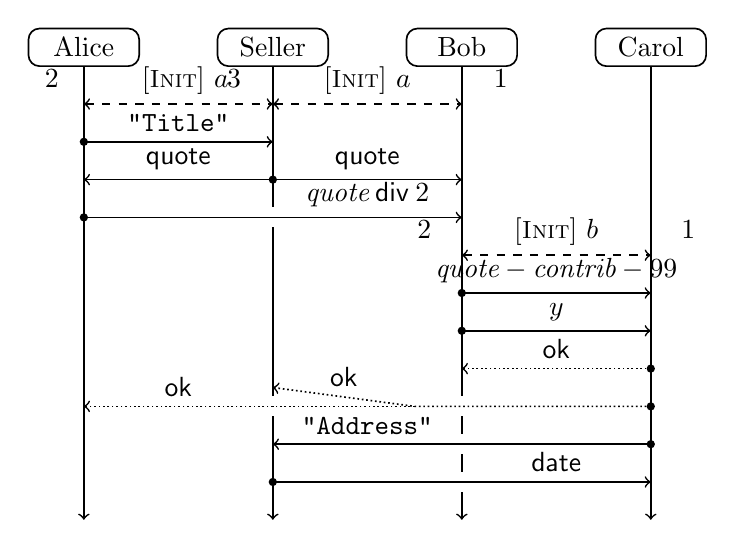
\begin{tikzpicture}[x=1.2cm,y=1.2cm,semithick]
  \node (alice) at (1, 5) [rectangle,draw,rounded corners,minimum
  width=4em] {\normalsize Alice};
  \node (seller) at (3, 5) [rectangle,draw,rounded corners,minimum
  width=4em] {\normalsize Seller};
  \node (bob) at (5, 5) [rectangle,draw,rounded corners,minimum
  width=4em] {\normalsize Bob};
  \node (carol) at (7, 5) [rectangle,draw,rounded corners,minimum
  width=4em] {\normalsize Carol};

  \node (x0) at (3, 3.2) {};
  \node (x1) at (5, 1.2) {};
  \node (x2) at (3, 1.2) {};
  \node (x3) at (5, 0.8) {};
  \node (x4) at (5, 0.4) {};

  \draw [->, draw] (alice) -- (1, 0);
  \draw [->, draw] (seller) -- (x0) -- (x2) -- (3, 0);
  \draw [->, draw] (bob) -- (x1) -- (x3) -- (x4) -- (5, 0);
  \draw [->, draw] (carol) -- (7, 0);

  \draw [<->, dashed, draw] (1, 4.4) -- node [above]
  {2~~~~~~~~~\rulename{Init}~$a$~~~~~~~~~~} (3, 4.4);
  \draw [<->, dashed, draw] (3, 4.4) -- node [above]
  {3~~~~~~~~~\rulename{Init}~$a$~~~~~~~~~1} (5, 4.4);

  \draw [->, draw]
  (1, 4) node [circle,fill,inner sep=0pt,minimum size=3pt] {}
  -- node [above] {\texttt{"Title"}} (3, 4);

  \draw [<->, draw] (1, 3.6)
  -- node [above] {$\mathsf{quote}$} (3, 3.6)
  node [circle,fill,inner sep=0pt,minimum size=3pt] {}
  -- node [above] {$\mathsf{quote}$} (5, 3.6);

  \draw [->, draw]
  (1, 3.2) node [circle,fill,inner sep=0pt,minimum size=3pt] {}
  -- (3, 3.2)
  -- node [above] {$\textit{quote} \mathbin{\mathsf{div}} 2$} (5, 3.2);

  \draw [<->, dashed, draw] (5, 2.8) -- node [above]
  {2~~~~~~~~~\rulename{Init}~$b$~~~~~~~~~1} (7, 2.8);

  \draw [->, draw]
  (5, 2.4) node [circle,fill,inner sep=0pt,minimum size=3pt] {}
  -- node [above] {$\textit{quote} - \textit{contrib} - 99$} (7, 2.4);

  \draw [->, draw]
  (5, 2) node [circle,fill,inner sep=0pt,minimum size=3pt] {}
  -- node [above] {$y$} (7, 2);

  \draw [->, draw, densely dotted]
  (7, 1.6) node [circle,fill,inner sep=0pt,minimum size=3pt] {}
  -- node [above] {$\mathsf{ok}$} (5, 1.6);

  \draw [->, draw, densely dotted]
  (7, 1.2) node [circle,fill,inner sep=0pt,minimum size=3pt] {}
  -- (4.5, 1.2)
  -- node [above] {$\mathsf{ok}$} (3, 1.4);

  \draw [->, draw, densely dotted]
  (4.5, 1.2) -- (3, 1.2) -- node [above] {$\mathsf{ok}$} (1, 1.2);

  \draw [->, draw]
  (7, 0.8) node [circle,fill,inner sep=0pt,minimum size=3pt] {}
  -- (5, 0.8)
  -- node [above] {\texttt{"Address"}} (3, 0.8);

  \draw [->, draw]
  (3, 0.4) node [circle,fill,inner sep=0pt,minimum size=3pt] {}
  -- (5, 0.4)
  -- node [above] {$\mathsf{date}$} (7, 0.4);
\end{tikzpicture}
\end{center}
\caption{An execution of the three buyer protocol.}\labelx{fig:threebuyers}
\end{figure}

Figure 1 depicts the execution of the above protocol where Bob asks Carol to collaborate (by delegating the remaining interactions with Alice and Seller) and the transaction terminates successfully. Note that row data(quote, quote div 2, quote-contrib-99) are represented by solid arrows, while labels(ok, quit ) are used to choose between different options and are shown in the diagrams by dashed arrow.
The first step to multiparty programming is using global types to specify the intended communication protocols. According to the scenario, two distinct global types are needed: one is $\cloG_a$among Alice, Bob and Seller and the other is $\cloG_b$ between Bob and Carol. For convenience, we use numbers to represent the role of each peer. In $\cloG_a$, 2 represents Alice, 3 represents Seller and 1 represents Bob, while in $\cloG_b$, Bob plays role 1 and Carol plays role 2. Following the definitions introduced before, a global description of this interaction is as follows:
\\[2mm]
{\small
\begin{minipage}{.5\textwidth}$%\begin{array}{@{}r@{~~}l@{}}
\cloG_a  = {} \\
\begin{array}[t]{ll@{~~~~}*{7}{l@{~~}}}
  & \nm{1} & 2 & \redsym & 3: & \multicolumn{2}{@{}l@{~~}}{\langle \kf{string}\rangle.} \\
  & \nm{2} & 3 & \redsym & \{1,2\}: & \langle \mathsf{int}\rangle. \\
  & \nm{3} & 2 & \redsym & 1: & \langle \mathsf{int}\rangle. \\
  & \nm{4} & 1 & \redsym & \{2,3\}: & \{\mathsf{ok:} & 1 \redsym 3:\langle \kf{string}\rangle.\\
  & \nm{5} & & & & & 3 \redsym 1: \langle \kf{date}\rangle .\End,\\
  & \nm{6} & & & & \phantom{\{} \mathsf{quit}: & \End\}
\end{array}$\end{minipage}\qquad\qquad
\begin{minipage}{.5\textwidth}$\cloG_b  = {} \\
\begin{array}[t]{ll@{~~~~}*{7}{l@{~~}}}
  & \nm{1} & 2 & \redsym & 1: & \langle \kf{int}\rangle .\\
  & \nm{2} & 2 & \redsym & 1: & \langle \cloT \rangle .\\
  & \nm{3} & 1 & \redsym & 2: & \{\mathsf{ok}:
  \End, \mathsf{quit}: \End\} \\
\end{array}$\end{minipage}
\[\cloT  = {\oplus} \langle\{2,3\},\{\mathsf{ok}:{!}\langle
3,\kf{string}\rangle.
{?}(3, \kf{date}). \End, \mathsf{quit}: \End\}\rangle\]
}

In Ga, line $\nm{1}$ denotes Alice sends a value in string type to Seller. Line $\nm2$ says Seller multicasts the same integer value to both Alice and Bob and line $\nm{3}$ says that Alice sends an integer to Bob. In lines $\nm{4-6}$, Bob has two sending options: ok or quit. The first option is Bob sends a string value to Seller and Seller answers with a date type; the second option is that there is no further interactions. 
Line $\nm 2$ in $\cloG_b$ represents the delegation of the capability specified by the session type $\T$ of channels from Bob to Carol. Type $\T$ contains all the types that Bob is going to do in Line$\nm{4-6}$. When Bob delegates his capabilities to Carol(sending type $\T$ to Carol), Carol knows what she is able to in the session, so that Carol behaves as Bob. Since the two specifications are independent, Alice does not have to know who would pass the capability.Note that the data from the global description is replaced by its type ("Title" and "Address" with string; quote, quote div 2 and quote-contrib-99 with int).

The next step is to specify the local type for each participant using the projection on global types.The local implementation for each of the participants of the global scenario is as follows:
\[\begin{array}{lll}
\pro{\cloG_\Ia}1&=& ?( 3,\kf{int}).?( 2,\kf{int}).\oplus\langle\{2,3\},\{\kf{ok}: !\langle 3 ,\kf{string}\rangle.?(3,\kf{date}).\End , \kf{quit}: \End\}\rangle\\
 \pro{\cloG_\Ia}2&=& !\langle 3,\kf{string}\rangle.?(3,\kf{int}).!\langle 1,\kf{int}\rangle.\&(1,\{\kf{ok}: \End , \kf{quit}: \End\})\\ 
 \pro{\cloG_\Ia}3&=& ?( 2,\kf{string}).!\langle \{1,2\},\kf{int}\rangle; \&(1,\{\kf{ok}: ?( 1,\kf{string}). !\langle 1 ,\kf{date}\rangle. \End , \kf{quit}: \End\})\\

\pro{\cloG_\Ib}1&=& ?( 2,\kf{int}).?( 2,\cloT).\oplus\anglep{2}{\{\kf{ok}: \End , \kf{quit}: \End\}}\\
\pro{\cloG_\Ib}2&=& !\langle 1,\kf{int}\rangle.!\langle 1,\kf{\cloT}\rangle.\&\anglep{1}{\{\kf{ok}: \End , \kf{quit}: \End\}}\\
\end{array}\]

The implementation above represents sessions from the view points of a single participant. With respect to the global type, the local view is obtained by removing the arrows, using ! and ? to indicate the sending and receiving actions as a sender or a receiver. By writing $\oplus$ when a process selects a label and $\&$ when offers different labels, the implementation includes branching and selection.
The types $\pro{\cloG_\Ib}1$ denotes the projection of participant 1 in the global type $\cloG_b$ and $\pro{\cloG_b}2$ denotes the projection of participant 2 in the global type $\cloG_b$ show a typical duality of session types. In these case, there will be no runtime error if the program is well-typed, so that duality ensures the properties of communication safety and session fidelity.















\end{document}